\documentclass{report}


\usepackage{alltt}
\usepackage{graphicx}
\usepackage{color}
\usepackage[small,bf]{caption}

\begin{document}
\title{EzQL: A new language for Event Stream Processing}
\author{Lu\'{\i}s Pureza}

\maketitle

\tableofcontents

\addtolength{\parskip}{\baselineskip}
\chapter{Introduction}
\label{chap:introduction}

Technology developments and its widespread adoption over the last
decades have significantly increased the demand for information
processing systems. Not only do we now need to process larger amounts
of information coming from everywhere, we must do it faster as
well. For some companies, obtaining results a few milliseconds earlier
may be a significant advantage over the competition. For others,
however, reacting immediately is of critical importance, as it
happens, for example, in the case of security breaches or nuclear
power plant malfunctions.

One particular class of applications, now referred to as Event Stream
Processing (ESP), has been the subject of much attention over the last
few years due to the technical challenges it presents. ESP
applications are characterized by dealing with a possible infinite
amount of data constantly flowing in to be processed as fast as
possible to continuously produce new and updated results that may
themselves be used to justify new decisions. It turns out that many
applications fit naturally in this model: financial analysis,
health-care monitoring, network intrusion detection, personnel and
product tracking through RFID devices, business monitoring and many
more.

Due to the inability of current technology to satisfy the increasing
demands from all these markets, computer scientists developed the
first Data Stream Management Systems (DSMS). Coming mostly from the
database community, these researchers intended to build a generic
engine that abstracted away all the low level details of managing
streams of data in high demanding scenarios, while retaining much of
the querying capabilities of regular Database Management Systems
(DBMS), so that they could be easily adapted to a multitude of
domains. It's no surprise then, that the first DSMSs inherited a SQL
dialect with some new extensions. Aurora [ref], with its boxes and
arrows graphical queries was the exception, but the operators it
provided still took inspiration from SQL. Later, when the first DSMS
hit the market, some emphasis was put on end-user interaction and some
applications began to include rule-based systems that allow the
developer to specify how he wants to react to events using Event
Condition Action (ECA) rules, a concept developed in the context of
active databases [ref]. At the same time, DSMS began to incorporate
features from Complex Event Processing (CEP) systems, that allowed the
user to detect complex patterns and correlations among the input
streams of data. This required adding new constructs into the query
language. Recently, some companies unhappy with declarative, SQL-like
languages, began to support procedural languages, more familiar to C
and Java programmers. Nowadays, each product includes its own flavor
of a SQL-like language with its own unique and esoteric extensions, or
a rule-based language, or a procedural language, or any combination of
these three. Besides the obvious issue created by the lack of a
standard, all this variety demonstrates that DSMS applications have
their own needs and a satisfactory end-user query language for them is
yet to be found.

To make matters worse, the semantics on many of these products
disagree in fundamental ways. In [ref], researchers analyzed how two
of the most prominent products from Oracle and StreamBase reacted in
the presence of simultaneous events. Surprisingly, they found that in
some scenarios, they are both wrong! Furthermore, they concluded that
this disparity may be blamed on the semantics employed by each
product. It also happens that many products consistently implement
inappropriate semantics. For example, as we will see in section
\ref{chap:soa}, DSMS typically provide ways of analyzing data newer
than some threshold: 3 minutes, 5 hours, 10 days, etc. However,
naively applying these constructs to answer a simple question such as
``Was the temperature above 20 $^{\circ}$C during any moment of the
last 5 minutes?'' will give wrong results. Will see why in chapter
\ref{chap:motivation}.

Despite these limitations, more and more organizations are adopting
DSMS and relying on them to process data coming from everywhere,
including core business processes. As a consequence, ESP applications
tend to grow and become more complex. However, it is our opinion that
languages available in currently existing products are not prepared to
support such large applications. It's just not the problem with the
semantics. Simply put, they were not designed for that. In chapter
\ref{chap:motivation} we will highlight many pitfalls of existing
solutions and even show a couple of perfectly reasonable queries in
the context of ESP applications, expressive in one sentence of
English, which are very difficult to implement. If they fail in those
situations, how could they handle complex applications?

The purpose of this internship is to design a new query language for
ESP systems. This new language combines powerful constructs, with some
innovative features that, we hope, should be a step in the right
direction to create a language that developers find rich, expressive
and coherent. The rest of this thesis is organized as follows:

\begin{itemize}
\item In chapter \ref{chap:soa}, we will expand on the previous
  paragraphs to detail the chap:soa and to show that art is indeed
  very subjective and multifaceted;
\item Chapter \ref{chap:motivation} discusses some limitations
  crippling currently available engines and provides some hints as to
  how they could be fixed;
\item Our proposal will then be introduced in chapter \ref{chap:ezql},
  first through the analysis of a few examples followed by a thorough
  discussion of all its features;
\item Further work and planning for the next semester will be the
  topic of chapter \ref{chap:future-work};
\item Finally, chapter \ref{chap:conclusion} concludes this document.
\end{itemize}

By the end of this document, it should be clear that not only current
technology will fail short of fulfilling the increasing needs of
costumers, but also that our proposal contains some interesting
characteristics that deserve further attention.

\chapter{State-of-the-art}
\label{chap:soa}

This section will analyze SQL dialects present in some industry
products for event processing - Coral8, StreamBase and Esper. Then,
StreamBase EventFlow, a method for creating queries visually through a
boxes and arrows interface will be discussed. Despite not involving
programming languages, it's important to study these alternatives
because, after all, they're trying to address the same problem. Next
comes Oracle Rules Manager with its rule-based paradigm for complex
event processing. We will conclude this chapter analyzing
MonitorScript, a procedural language developed by Progress Apama to
overcome the limitations imposed by SQL.

\section{SQL-based languages}
\label{sec:sql}

The most popular way of writing queries is through a declarative,
SQL-based language. Products adopting this solution include Coral8
[ref], StreamBase [ref] and Esper [ref]. As explained in the
introduction, this comes as a result of all the effort the database
community has put into creating the first ESP engines. Currently there
is no standard for a query language designed specifically for these
applications which means each vendor has their own. Fortunately,
they're all very similar. The simplest things can be done exactly as
in regular SQL:

\begin{verbatim}
INSERT INTO PriceMicrosoft
SELECT *
FROM StockTrades
WHERE symbol = 'MSFT'
\end{verbatim}

This query looks for tuples where the field \verb=symbol= equals
``MSFT'' arriving at the stream \verb=StockTrades= and adds them to
the \verb=PriceMicrosoft= stream. It's just a simple filter.

One feature that assumes particular importance in the context of ESP
is the concept of window. Windows allow developers to consider only
part of a stream and make computations over it. In particular, it
becomes possible, for example, to calculate the most expensive order
among the last million, or the average of Microsoft's stock prices
over the last 3 hours, as the following example shows:

\begin{verbatim}
INSERT INTO AvgPriceMicrosoft
SELECT avg(price)
FROM StockTrades KEEP 3 HOURS
WHERE symbol = 'MSFT'
\end{verbatim}

It's possible to customize the retain policy and keep, for example,
the 10 largest updates based on their price, the 10 last updates per
company or simply to keep everything.

The window defined in the previous example is a \emph{sliding}
window. Sliding, in this context, refers to how and when the elements
in the window expire. In these kinds of windows, tuples are removed
from the window as they become too old or new tuples arrive. An
alternative is \emph{jumping} windows, where tuples are appended to
the window and then, when the oldest element was supposed to be
removed, all of them expire at the same time, the window becomes empty
and the cycle begins all over again. This way, it's possible to find
out the largest price attained by Microsoft stocks over the last hour,
the hour before and so on.

All the examples in this section were written in Coral8 Continuous
Computation Language (CCL). Nonetheless, all the other systems in this
section provide similar features albeit with different syntax. In
fact, there have been talks about creating a standard language lately,
an idea that was met with some skepticism by some vendors and users
that don't like SQL anyway and opted for other approaches [ref].

With the undeniable increasing relevance of ESP and the predominance
of SQL-based languages in currently-available products, it is
important to analyze the limitations of these languages. After all, it
doesn't make sense to build yet another programming language if the
existing ones are good enough. This will be the topic of the next
chapter.

\section{Building queries visually with StreamBase's EventFlow}
\label{sec:eventflow}

StreamBase employs an alternative, more user-friendly, way of building
queries. Instead of writing code, the user can design queries
visually, by arranging boxes in a canvas and connecting them with
arrows. Boxes represent operators that receive data coming from other
operators or directly from the input streams, process the data
according to its semantics and send the results to be handled by other
operators, or to the world as the output of the whole operation. An
example is shown in figure \ref{fig:eventflow-sample}.

\begin{figure}[htbp]
  \centering
  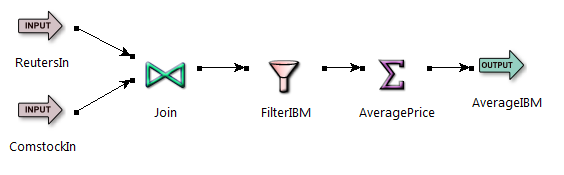
\includegraphics[width=\textwidth]{eventflow.png}
  \caption{This diagram represents a simple query where two streams
    are joined, non IBM tuples are filtered-out, and then the average
    of IBM stock prices over the last 5 minutes is sent to the
    output.}
  \label{fig:eventflow-sample}
\end{figure}

Some of the most important operators are:

\begin{description}
\item [Aggregate] Computes aggregate operations over windows of
  tuples. Supports the option to partition tuples into sets and then
  apply the aggregation over each individual set, much like a SQL
  GROUP BY statement;
\item [Filter] Discards some tuples from the input stream based on a
  predicate. Performs the same function as a SQL WHERE statement;
\item [Gather] Receives tuples from two or more streams and
  concatenates those with the same key. The resulting tuple values may
  be direct copies from the original tuples or the result of applying
  some expression to these;
\item [Join] Similar to SQL joins, this operator pairs tuples coming
  from two streams that match a given condition and outputs a new
  tuple whose fields may be specified by the user. In general, joining
  two infinite streams may require keeping all tuples from both
  streams in memory. To avoid problems later on, the user must specify
  timing constraints regarding matching tuples saying, for example,
  that they must arrive withing 60 seconds of each other;
\item [Map] Similar to the first part of a SELECT statement, this
  operator transforms a tuple --- possibly discarding or adding new
  fields along the way ---, and sends it downstream;
\item [Pattern] Instructs the engine to look for complex events. This
  is a feature borrowed from Complex Event Processing and will be
  discussed below;
\item [Union] Acts as a multiplexer, connecting many input streams to
  a single output stream, to where all tuples are sent. Similar to the
  SQL UNION statement.
\end{description}

It's clear that most of these operators have SQL counterparts. There
are a few things that can be done in EventFlow but not in StreamSQL
[ref], but they're just small details, nothing that changes the
developer's way of thinking. It's then mostly a matter of taste ---
not power ---, to choose between StreamSQL and EventFlow.

\section{Oracle rules}
\label{sec:orm}

Oracle Rules Manager (ORM) embraces a completely different
paradigm. Instead of writing queries, the user creates rules that are
made of three parts. The first, the event type, instructs the system
to trigger the rule only when an event of that type occurs. The
second, the condition, is a predicate that is compared against the
event. If they match, the third part, the action --- a PL/SQL
procedure ---, is executed.

Conceptually, a rule has the following format:

\begin{verbatim}
ON   <event>
IF   <condition>
THEN <action>
\end{verbatim}

The following example shows a simple rule:

\begin{verbatim}
ON   StockTick(symbol, price, volume)
IF   symbol = 'MSFT' and price > 100
THEN buyStocks(symbol)
\end{verbatim}

The event shown above represents a stock update received from some
external source. These are the simplest kind of events, also called
\emph{primitive} events. ORM also supports \emph{composite} events
that are defined as combinations of other events. For example, it is
possible to define a composite event that occurs when Microsoft shares
drop by 10\% and, less than 5 minutes later, IBM shares gain 2\%. To
be more specific, the following types of combinations are supported:
\begin{description}
\item [Sequencing] Specifies the order between events, i.e., event A
  must occur before event B;
\item [Negation] Checks for the non-occurrence of some event. Useful
  to raise exceptions when business rules are violated;
\item [Set semantics] Allows combining events with the AND operator to
  specify that all of them must occur for the composite event to occur
  as well;
\item [Any N] Checks for the occurrence of at least N children events;
\item [Collection] Combines a set of primitive events based on some
  common properties. Could be used, for example, to detect all
  costumers who withdrew more than \$1000 from their bank accounts
  during the past 24h.
\end{description}

ORM comes with a GUI utility to simplify the rules creation
process. This is necessary because creating a rule the hard way is a
daunting task that involves writing SQL queries containing XML blocks
containing SQL snippets inside. Still, there are situations when one
needs to avoid these utilities and work with real code, situations
where a simpler configuration process would be desirable.

The biggest disadvantage of rule-based languages comes from the
paradigm itself. While they may be effective for detecting complex
patterns of events, they are not so good when it comes to actually
processing the data. Built-in combinators provide some aggregation
functions, but these will seem basic for companies in need to
implement proprietary analysis algorithms. Also, PL/SQL is arguably
not a language suited for complex application development.

One other issue that plagues these systems is the difficulty to reason
about their runtime behavior. As the number and complexity of rules
increases, an event may trigger more than one rule and these rules may
themselves trigger other rules, resulting in a cascading process that
may never end. This behavior makes the applications more difficult to
understand, to the point where even adding or removing a simple rule
may have unpredictable effects. These kinds of non-linear interactions
are discouraged by Software Engineering best-practices and thus, the
decision to use rule-based systems for building large applications
must be carefully pondered. To be fair, Oracle Rules Manager provides
constructs to deal with simultaneous triggering rules, but the problem
doesn't go away: only now the developers will be to blame when things
go wrong.

\section{Apama's MonitorScript}

When ESP solutions left the academia to meet the real world, many
users argued that SQL was ill-suited for many information processing
tasks. MonitorScript (MS) is Apama's response to these complains.

Deriving from the procedural family of programming languages, MS
programs look a lot like Java programs. However, the most important
and unique feature it includes was borrowed from Erlang: the process
model based on having many little \emph{processes} that execute in
parallel and communicate with each other through messages. In MS,
these entities are called \emph{monitors}. A monitor is an event
processing agent that basically sets up an arbitrary number of
\emph{listeners} that await for the occurrence of events. When one
matching event arrives, monitors process it. Monitors can also send
events to each other, through the \emph{route} statement.

Last but not least, monitors can have state. This means that instead
of writing a SQL query to capture the state of the system, MS updates
the state incrementally as the computation moves forward. The downside
is that, for simple things, SQL queries will definitely be easier to
understand, because a SQL query \emph{is} its intention while, in a
procedural program, the big picture is not always that clear.

To get a feeling for the language, here is a small MonitorScript
snippet:

\begin{verbatim}
monitor ProcessMarket {
    // Keep the last price per company
    dictionary <string, int> lastPerCompany;

    action onload {
        Tick tick;
        on all Tick(): tick {
           processTick(tick);
        }

        on all PriceRequest(): ev {
            processPriceRequest(ev);
        }
    }

    action processTick(Tick tick) {
        lastPerCompany[tick.sym] := tick.price;
        route TickAck(tick.sym);
    }

    action processPriceRequest(PriceRequest ev) {
        if (lastPerCompany.hasKey(ev.sym)) then {
            route PriceReply(ev.sym, lastPerCompany[ev.sym]);
        }
    }
}
\end{verbatim}

This listing declares one monitor (\verb=ProcessMarket=), that waits
for \verb=Tick= and \verb=LastPriceRequest= events. When it receives a
new \verb=Tick= update, it keeps the price reported in a dictionary,
indexed by the company's symbol and replies with a \verb=TickAck=
message. When it receives a \verb=PriceRequest=, it fetches the last
price from the dictionary and sends a \verb=PriceReply= message.

Note the need to create request, reply and acknowledgement messages
when what one really wants to do is to perform a method invocation
between different monitors. Indeed, the runtime system could provide
some kind of remote procedure call mechanism and handle the low-level
details by itself.

MS and SQL are at opposite ends of the programming language
spectrum. While is simplifies a lot of tasks that don't naturally fit
into SQL, MS also looses all the querying capabilities that made SQL
and its derivatives popular for data processing.

\chapter{Simple questions, complex answers}
\label{chap:simple-questions-complex-answers}

In this chapter we are going to discuss some simple queries that are
very complex to express using existing SQL dialects for ESP
systems. We will try to understand the reasons for this difficulty and
propose solutions to eliminate it.

\section{The IBM problem}

The first problem is also the simplest. You are given a stream that
receives events from the financial market containing company symbols
and their corresponding stock prices. With this stream, you need to
answer the following question: ``Were IBM actions above \$70 during
any moment of the last 5 minutes?''.

This seems to be a great use-case for temporal sliding windows
discussed in chapter \ref{chap:soa}. Unfortunately, the semantics of
these windows are not appropriate here. To see why, suppose that, at
10:54, the system receives a notification reporting that IBM actions
were worth \$71 and, 2 minutes later, it receives another event
informing that the price decreased to \$69. Suppose further that no
other events arrived until the question is posed, at 11:00 (of the
same day). Given these assumptions, any human would answer the obvious
``yes'', because IBM actions were valued at \$71 between 10:54 and
10:56 --- well inside the 5 minutes window. However, existing engines
ignore what happens between events. It's like the price is undefined
between two consecutive updates. Thus, the engine will completely
ignore the \$71 notification, because it lies outside the 5 minutes
window, as figure \ref{fig:outside-window} shows.

\begin{figure}[htbp]
  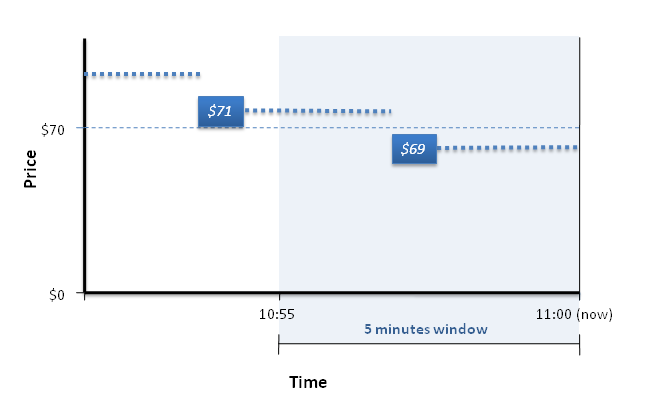
\includegraphics[width=\textwidth]{outside-window.png}
  \caption{Evolution of IBM stock prices in the scenario described in
    the text. Values in blue boxes represent the two events received
    at 10:54 and 10:56. As you can see, the first event lies outside
    the 5 minutes window and thus, will be ignored by the system. The
    dotted blue lines illustrate the fact that prices remain constant
    until the next update, an assumption made by humans that the
    system is unaware of.}
  \label{fig:outside-window}
\end{figure}

Note that these semantics will result in wrong results for many other
queries. For example, if you try to calculate the average price during
the last 5 minutes using a simple sliding window, the engine will
return \$69, despite the fact that the price was \$71 during 1 of
those 5 minutes.

A solution to this problem implemented in Coral8 CCL can be seen in
Appendix [ref]. The algorithm creates two windows: the 5 minutes
window and another window that will contain the newest event older
than 5 minutes (i.e., the event that most recently expired from the 5
minutes window). Then, we perform a LEFT OUTER JOIN between both
windows (UNION would be more appropriate, but Coral8 doesn't support
it) and check if the maximum price in any of these windows is greater
than 70. Clearly, although it is possible to write the correct
solution, it should be easier to do so.

To solve this problem in a more effective way, one needs to instruct
the engine about what happens between events --- i.e., we need to tell
it that stock actions retain their values until the next update. In
general though, we could specify any mathematical function that, for a
given time and history of values, returns an approximation to the
current value. With this change, the evolution of price becomes a
continuous function (shown in figure \ref{fig:outside-window} as a
dotted blue line) that is always defined for any given
timestamp. Answering the original question now becomes equivalent to
checking if this continuous function is above \$70 anywhere in the
last 5 minutes of its domain.

This same problem was posed on an online community where researchers
and vendors participate [ref]. It generated a lengthy (more than 60
messages), interesting and sometimes funny debate. Several vendors
replied --- including Oracle, Aleri, Coral8 and Esper ---, and tried
to find a good solution using their products, but they failed to do
so, because their solutions were too complex, inneficient or just
plain wrong. In the end, some participants concluded this was not an
event processing problem anyway because it envolves state and tried to
dismiss it as irrelevant, while others argued that queries like these
show up every day and if ESP engines can't solve them, their
usefulness is reduced.

\section{More windows}

Suppose that IBM actions were worth more than \$70 during some
interval and you want to know what was the average of their price
during that interval. Solving this problem using current technology is
not so difficult. Most ESP products include some kind of event
detection feature that allows the search for patterns of events. To
obtain an answer, we could find the event where IBM stocks passed the
\$70 mark, then find all the events where the price stayed above that
threshold and finally, find the event where they descended below
\$70. With all these events, we could then proceed to calculate the
average price.

There are two problems with this approach. The first is that the
detection of the boundaries of this interval may itself involve the
detection of another complex pattern. For example, to discover the
event where the price rose above \$70, one needs to compare some event
with the one that preceded it. The second problem is that these
complex event detection features work by first detecting the pattern
and then processing it. Thus, while the price remains above \$70, the
engine keeps all the events in memory and only when the price goes
below that mark will it proceed to calculating the average. This is
suboptimal, because the engine could keep a temporary sum of the
prices and a temporary count of the number of events received. These
two numbers are enough to generate the average and thus, the events
themselves could be discarded immediately.

In the previous section [ref] we concluded that the evolution of stock
prices could be seen as a continuous function. Then, conceptually,
solving this problem should be as easy as writing a continuous query
that calculates the average \emph{while} the price is greater than
\$70.

\section{Spoiled products detection}
Another class of problems that are reasonable in the context of ESP
systems but are difficult to solve by current systems are those where
the developer needs to know for how long was a certain condition true
(or false). For example, imagine the following scenario, attributed to
Andrew Witkowski from Oracle: a factory has three rooms, every room
has at least one humidity sensor and one temperature
sensor. Furthermore, products contain a RFID tag that is read by RFID
sensors placed at the entrance and exit of each room. All these
sensors send their readings to a DSMS that needs to answer the
following question: ``Which products stayed more than 10 minutes
(overall, not consecutive) at more than 20 ºC and 80\% of
humidity?''. These products are spoiled and mustn't be sold.


\section{Variable-sized windows}

We've seen before that ESP systems provide many windowing facilities
on top of regular SQL -- sliding windows, jumping windows, windows per
groups, etc. However, all these windows share a common limitation:
their sizes are fixed. Suppose you have a new stream whose events
represent requests to calculate the average price of the last N stock
updates for some company. Usually, this would be solved by creating a
window that keeps the last N events for that company. Imagine,
however, that N is a field of the request --- i.e., the client decides
how many events to use in the calculation ---, with the restriction
that it must be smaller than some arbitrary number (otherwise it would
be necessary to keep everything in memory). Unfortunately, we don't
know of any way to solve this using SQL dialects in existing products,
because its not possible to create variable-sized windows even if they
are contained inside a bigger window.

Some may argue that this is not event processing at all because it
involves requests that are better handled by a traditional
DBMS. Still, these scenarios may be more frequent than one thinks and
it doesn't seem like it's complex to implement anyway.





TODO:
 - Problema da fabrica (explicar o que seria necessario mudar para a humidade)
 - malloc e free (aggregators must be used with windows)
 - Problema do leilao



 It's not our purpose to claim that SQL, in general, is not
well-suited for these kinds of applications. On the contrary: SQL and
its derivatives have been successfuly employed in databases for over
30 years and their decline is unlikely to happen any time
soon. However, we believe that, in order to solve these problems, one
needs new data types, operators and different semantics, and the resulting language 

 and that results in a
new language bearing little resemblance with current ones.



 It may
thus seem imprudent to claim that SQL is not well-suited for ESP and
such a statement must be accompanied with valid
arguments. Fortunately, it is quite easy to understand, intuitively,
the problems with this approach. First, experience tells that SQL
queries easily become overly complex and hard to understand ---
especially when they begin to include subqueries or perform analytical
operations now part of the SQL standard. Second, SQL's declarative
nature doesn't always map well with the way programmers
think. Sometimes, things that are simple to do in C or Java become
ugly hacks when translated to SQL, because SQL, despite being
Turing-complete, just wasn't made to compete with those languages. We
will develop these arguments while exploring a simple example (adapted
from [ref]).

\section{The online auction}

Robay, a fictional online auction company, is experimenting with a
DSMS to manage auctions. In their setup, they have three streams:

\begin{itemize}
\item \verb=OpenAuction(itemId, start_price)=: New tuples arriving
  on this stream signal the beginning of a new auction;
\item \verb=ClosedAuction(itemId)=: Signals the end of an auction;
\item \verb=Bid(itemId, bid_price)=: Updated when there is a new bid
  for an ongoing auction.
\end{itemize}

Information on sellers and buyers has been omitted because it won't be
necessary to illustrate our point. One of the first queries Robay
developers wrote returns, for each closed auction, its item id along
with the price offered in the winner bid:

\begin{verbatim}
-- Unite Bid with OpenAuction
ItemPrices:
    SELECT itemID, bid_price as price
    FROM   Bid
    UNION ALL
    SELECT itemID, start_price as price
    FROM   OpenAuction

-- Get the current price for each product
CurrentPrice:
    SELECT    P.itemID, Max(P.price) as price
    FROM      ItemPrices P
    GROUP BY  P.itemID

-- Get the product and final price for each closing auction
ClosingPriceStream:
    SELECT   Rstream(P.itemID as itemId, P.price as price)
    FROM     ClosedAuction [Now] C, CurrentPrice P,
    WHERE    C.itemID = P.itemID
\end{verbatim}

This solution uses regular SQL extended with windowing constructs and
should be pretty easy to understand. Despite being so straightforward,
there are a few places where it could be improved. First of all,
notice that besides the \verb=ClosingPriceStream= --- the desired
result ---, two other temporary streams had to be created. They are
not strictly necessary and their code could be directly inserted in
the \verb=FROM= clause of the \verb=ClosingPriceStream=, but that
would quickly result in unreadable code. To avoid creating big and
complex queries, developers partition them into smaller ones connected
by temporary streams. Thus, streams end up being used as variables to
store the intermediate results of computations. But streams aren't a
suitable replacement for all kinds of variables. In procedural
programming languages, programmers can choose among primitive
variables (int, float, string, \dots), arrays, dictionaries, lists and
sets among others, to manage information. Furthermore, Object-Oriented
Programming brought classes and objects to the table, important not
only to keep information in an organized way, but also because they
allow developers to think in terms of the real world and model objects
and the relationships between them. Certainly, streams and tables
alone could be used to simulate all these kinds of constructs, but
they're just not the right tool for \emph{every} job.

Second, notice the query for the \verb=CurrentPrice= stream. To find
the current price, it first finds the starting price, then all the
prices from later bids and finally it chooses the largest, which is
also the latest. Notice how the query builds, implicitly, the current
state of each item by processing each event that affects it. This is a
common pattern in SQL dialects for ESP and it works because the state
is dictated by the events. What this means is that if you start from
the same initial state and follow, one by one, the events that affect
this state, you always arrive to the same result in the end, just like
in a finite state machine. While this approach works, it soon becomes
tedious to write queries like these, specially if the state may be
affected by many different types of events interacting in complex
ways. This query would be greatly simplified if there was some way to
manage the state explicitly, by defining \verb=Item= objects with
properties like \verb=currentPrice= to hold the state of each item and
use these objects in queries, just like regular tuples. Moreover,
these objects and their properties could be automatically managed by
the system, thus relieving the programmer from lower-level tasks.

Third, notice the \verb=WHERE= predicate in the last query. This
predicate contains one inner join and should be clear for any SQL
programmer. The problem is that this join hides an important fact
about the system being modeled: objects have relationships. Auctions
have one item and items have zero or more bids. Relationships are not
new to the database community: DBMSs have embraced and supported them
for years. But database relationships are still considered too
low-level by most programmers, who are used to think in terms of
objects instead of meaningless identifiers. This is one reason why
Object-Relational Mapping (O/RM) has flourished in the last few
years. If the developer could, somehow, model these relationships, the
system would be able to enrich the objects mentioned in the previous
paragraph with pointers to the related objects and manage these
pointers automatically. With these changes, the last query would
become much more explicit and read something along the lines of ``For
every closed auction, get the current price, category and id of its
item''.

It may seem that these issues aren't as bad as we're making
them. After all, the queries above are still easy to understand. Note
however, that the example is also very short. As explained in the
introduction, more and more code like this is being written like this
every day by organizations that rely on DSMS to manage their business
processes. As the code base grows, this mismatch between what
developers want and what the systems have to offer becomes more
evident to the point where, eventually, code becomes unmaintainable
and needs to be abandoned.


To conclude this chapter, it should be said SQL has some benefits. For
simple things, its declarative nature makes it very expressive. After
all, queries represent, almost in English, the intention of the
developer. Also, SQL querying capabilities are very powerful and excel
in many data processing tasks. It is understandable then, that an
alternative language should take some inspiration from SQL and borrow
some features to provide equally powerful constructs.


\chapter{The EzQL query language}
\label{chap:ezql}

In this chapter we present EzQL, our language designed to overcome 

\chapter{Future work}
\label{chap:future-work}

\chapter{Conclusion}
\label{chap:conclusion}

\appendix
\chapter{Solutions in Coral8}

This appendix contains solutions to some of the problems discussed in
chapter \ref{chap:simple-questions-complex-answers}. We can't claim
these are the best solutions nor the smallest, but they were all
proposed/reviewed by Coral8 personnel. We added a few comments to help
the understanding of the code. Still, if you find yourself staring at
the code and thinking ``this can't be that hard!''\ldots that's the
point.

\section{The IBM problem}

\begin{verbatim}
-- Algorithm:
--
-- Keep two windows: one for the last 5 seconds of data, and another with
-- the newest event that is older than 5 seconds (i.e., the one that
-- expired last from the first window). Then, join both windows (UNION
-- would be better, but Coral8 doesn't support it) and check if the
-- max of prices in any of the two windows is > $70.

CREATE INPUT STREAM StreamIn
SCHEMA (
   symbol STRING,
   price  INTEGER
);

-- Keep the events from the last 5 seconds.
CREATE WINDOW Last5Secs
Schema (
  symbol STRING,
  price  FLOAT
) KEEP 5 Seconds
INSERT REMOVED ROWS INTO Expired;

 -- Insert the events into the window.
INSERT INTO Last5Secs
SELECT *
FROM StreamIn;


-- Keeps the previously expired event from Last5Secs (one per symbol)
CREATE WINDOW Expired
Schema (
  symbol STRING,
  price  FLOAT
) KEEP LAST PER symbol;


-- For each symbol, true means its stocks were at > $70 during any moment
-- of the last 5 seconds, false means otherwise.
CREATE WINDOW Result
Schema (
  symbol STRING,
  result BOOLEAN
) KEEP LAST PER symbol;

-- Join both windows and check if the max of any of them is > $70
-- This would be prettier with UNION
--
-- Note: When events expire, this generates two events: one before
--       the expiration and another after.
INSERT INTO Result
SELECT L.symbol,
      IF max(coalesce(max(L.price), 0), coalesce(max(E.price), 0)) > 70
       THEN TRUE
        ELSE FALSE
      END
FROM Last5Secs AS L LEFT OUTER JOIN Expired AS E
      ON L.symbol = E.symbol
GROUP BY L.symbol;
\end{verbatim}

\section{The factory problem}

This is just a simplification of the original problem. In particular,
it doesn't handle humidity and it's assumed that rooms have a single
temperature sensor.

\begin{verbatim}
-- Algorithm:
--
-- - Always maintain an explicit counter per product containing
--   the number of seconds the product spent at > 20 degrees.
--   This counter also contains the time the product was last
--   updated (last_update).
--
-- - When a product swicthes rooms, if the temperature in the
--   previous room was > 20, add now() + last_update to the
--   counter and replace the previous last_update with now();
--
-- - When the temperature in a room changes, if the previous
--   temperature was > 20, add now() + last_update to the
--   counter and replace the previous last_update with now();
--

CREATE INPUT STREAM entries
SCHEMA (
   product_id STRING,
   room_id STRING
);

CREATE INPUT STREAM temp_readings
SCHEMA (
   room_id STRING,
   temperature INTEGER
);


-- Holds the last two entries per product
CREATE WINDOW ProductRoom
Schema (
   product_id STRING,
   room_id STRING
) KEEP 2 ROWS PER product_id;


INSERT INTO ProductRoom
SELECT *
FROM entries;


-- Holds the last two temp_readings per room
CREATE WINDOW RoomTemperature
Schema (
   room_id STRING,
   temperature INTEGER
) KEEP 2 ROWS PER room_id;


INSERT INTO RoomTemperature
SELECT *
FROM temp_readings;

CREATE LOCAL STREAM OnExit
SCHEMA (
   product_id STRING,
   old_room_id STRING
);


-- When a product leaves a room, generate an event containing the
-- product and the old room.
INSERT INTO OnExit
SELECT entries.product_id, ProductRoom.room_id
FROM entries LEFT OUTER JOIN
 ProductRoom ON entries.product_id = ProductRoom.product_id
WHERE entries.room_id != ProductRoom.room_id;


CREATE LOCAL STREAM OnTemperatureChange
SCHEMA (
   room_id STRING,
   old_temperature STRING
);


-- When the temperature changes, generate an event containing the
-- room and the old temperature
INSERT INTO OnTemperatureChange
SELECT temp_readings.room_id, RoomTemperature.temperature
FROM temp_readings LEFT OUTER JOIN
 RoomTemperature ON temp_readings.room_id = RoomTemperature.room_id
WHERE temp_readings.temperature != RoomTemperature.temperature;

-- Per each product, maintain a counter with the time the product
-- spent above 20 degrees and the last time this counter was updated
CREATE WINDOW ProductTemperatureCounter
Schema (
   product_id    STRING,
   time_above_20 INTERVAL,
   last_update   TIMESTAMP
) KEEP LAST PER product_id;

-- Initialize this counter
INSERT INTO ProductTemperatureCounter
SELECT product_id, 0 seconds, NOW()
FROM entries
WHERE room_id = "A";

-- Every time the product leaves the room, checks if the temperature in
-- the old room was > 20 and updates the counter of that product
INSERT INTO ProductTemperatureCounter
SELECT E.product_id, IF T.temperature > 20
                      THEN time_above_20 + now() - C.last_update
                      ELSE time_above_20
                    END, now()
FROM OnExit as E, RoomTemperature as T, ProductTemperatureCounter as C
WHERE E.old_room_id = T.room_id
 AND E.product_id = C.product_id;

-- Every time the temperature changes, checks if the previous temperature
-- was > 20 and updates the counters of all the products in that room
INSERT INTO ProductTemperatureCounter
SELECT R.product_id, IF T.old_temperature > 20
                      THEN time_above_20 + now() - C.last_update
                      ELSE time_above_20
                    END, now()
FROM OnTemperatureChange as T, ProductRoom as R, ProductTemperatureCounter as C
WHERE T.room_id = R.room_id
 AND R.product_id = C.product_id;
\end{verbatim}

\end{document}